\documentclass[10pt]{beamer}
\usetheme[
%%% option passed to the outer theme
%    progressstyle=fixedCircCnt,   % fixedCircCnt, movingCircCnt (moving is deault)
  ]{Feather}
  
% If you want to change the colors of the various elements in the theme, edit and uncomment the following lines

% Change the bar colors:
%\setbeamercolor{Feather}{fg=red!20,bg=red}

% Change the color of the structural elements:
%\setbeamercolor{structure}{fg=red}

% Change the frame title text color:
%\setbeamercolor{frametitle}{fg=blue}

% Change the normal text color background:
%\setbeamercolor{normal text}{fg=black,bg=gray!10}

%-------------------------------------------------------
% INCLUDE PACKAGES
%-------------------------------------------------------

\usepackage[utf8]{inputenc}
\usepackage[english]{babel}
\usepackage[T1]{fontenc}
\usepackage{helvet}

%% Brazilian encoding :
%\usepackage[brazilian]{babel} % English language/hyphenation
%\usepackage[T1]{fontenc} % Use 8-bit encoding that has 256 glyphs
%\usepackage[utf8]{inputenc}

% Symbols :
\usepackage{gensymb}

% Pictures management :
\usepackage{caption}
\usepackage{graphicx} % to insert png
\usepackage{adjustbox} % for better figure positionning
\usepackage[space]{grffile} % allow space in figure path
\usepackage{float}% Prevent pictures to moves to next page automatically

%-------------------------------------------------------
% DEFFINING AND REDEFINING COMMANDS
%-------------------------------------------------------

% colored hyperlinks
\newcommand{\chref}[2]{
  \href{#1}{{\usebeamercolor[bg]{Feather}#2}}
}

%-------------------------------------------------------
% INFORMATION IN THE TITLE PAGE
%-------------------------------------------------------

\title[] % [] is optional - is placed on the bottom of the sidebar on every slide
{ % is placed on the title page
      \textbf{Weightless Neural Network for Building's energy consumption classification}
}

\subtitle[]
{
      \textbf{}
}

\author[Guillaume Jeusel]
{      Guillaume Jeusel \\
      {\ttfamily jeusel.guillaume@gmail.com}
}

\institute[]
{
      Universidade Federal do Rio de Janeiro\\
      Palestra NCG013 ``Priscila Lima''\\
  
  %there must be an empty line above this line - otherwise some unwanted space is added between the university and the country (I do not know why;( )
}
\date{\today}

%-------------------------------------------------------
% THE BODY OF THE PRESENTATION
%-------------------------------------------------------

\begin{document}

%-------------------------------------------------------
% THE TITLEPAGE
%-------------------------------------------------------

{\1% % this is the name of the PDF file for the background
\begin{frame}[plain,noframenumbering] % the plain option removes the header from the title page, noframenumbering removes the numbering of this frame only
  \titlepage % call the title page information from above
\end{frame}}


\begin{frame}{Content}{}
\tableofcontents
\end{frame}

%-------------------------------------------------------
\section{Introduction}
%-------------------------------------------------------
\subsection{Dataset presentation}
\begin{frame}{Introduction}{Dataset presentation}
%-------------------------------------------------------

\begin{itemize}
  \item Dataset from\chref{https://archive.ics.uci.edu/ml/datasets/Energy+efficiency}{UCI}:
    \begin{minipage}{0.95\linewidth}
        \centering\medskip
        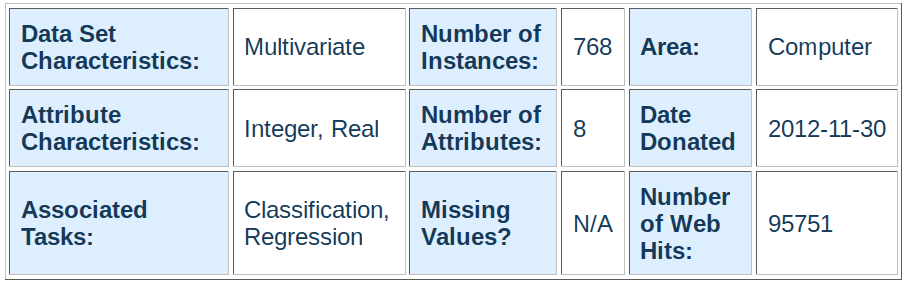
\includegraphics[scale=0.35]{../figures_trabalho_final/resume_dataset.png}
        \captionof{}{Dataset Summary}
        \medskip
    \end{minipage}
    \item Those registers are obtained by simulating 12 different building
        shapes with\chref{http://logiciels.i3er.org/ecotect.html}{Ecotect}.
    \item Using building energy simulation software may
        provide reliable solutions to estimate the Energy Load. However
        this can be very time-consuming and requires user-expertise.
\end{itemize}
\end{frame}

%-------------------------------------------------------
\begin{frame}{Introduction}{Dataset presentation}
\begin{itemize}
  \item Hence, in practice many researchers rely on machine learning tools
      to study the effect of various building parameters because this is
        easier and faster.

  \item energy-efficiency.csv file contains :\\\medskip
    \begin{tabular}{llcc}
      \hline
      Var. & Var. meaning & N possible values & Unit \\
      \hline
      X1 & Relative Compactness & 12 & None \\
      X2 & Surface Area & 12 & $m^2$\\
      X3 & Wall Area & 7 & $m^2$\\
      X4 & Roof Area & 4 & $m^2$\\
      X5 & Overall Height & 2 & $m$\\
      X6 & Orientation & 4 & Unknown\\
      X7 & Glazing Area & 4 & $m^2$\\
      X8 & Glazing Area Distribution & 6 & None \\
      y & Total Load & 636 & Unknown \\
    \end{tabular}
\end{itemize}
\end{frame}

%-------------------------------------------------------
\subsection{Purpose}
\begin{frame}{Introduction}{Purpose}
\begin{itemize}
  \item \textbf{Purpose} : using machine learning WiSARD's algorithm
    to predict building energy classification according to their geometry.

\begin{columns}[T] % align columns
\begin{column}{.48\textwidth}
    \begin{minipage}{0.95\linewidth}
        \medskip\bigskip\medskip
        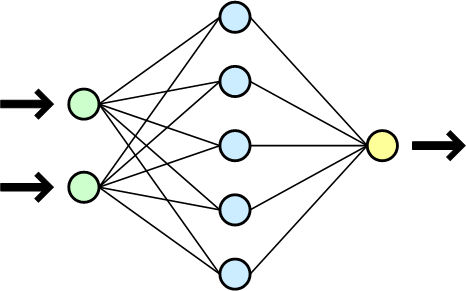
\includegraphics[scale=0.25]{../figures_trabalho_final/Neuralnetwork.png}
        \captionof{}{\textbf{Entries}: variables converted into binaries\\
        \textbf{Output}: Class of building}
        \medskip
    \end{minipage}
\end{column}%
\begin{column}{.48\textwidth}
    \begin{minipage}{0.95\linewidth}
        \medskip
        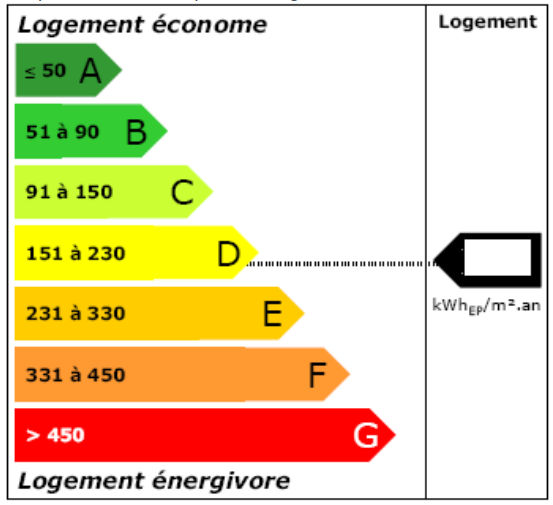
\includegraphics[scale=0.25]{../figures_trabalho_final/classification_consomation.png}
        \captionof{}{Classes of building}
        \medskip
    \end{minipage}
\end{column}%
\end{columns}

\end{itemize}
\end{frame}

%-------------------------------------------------------
\subsection{Data Formatting}
\begin{frame}{Introduction}{Data Formatting}
\begin{itemize}
  \item \textbf{Different steps} :
\end{itemize}
    \begin{minipage}{0.95\linewidth}
      \flushleft
      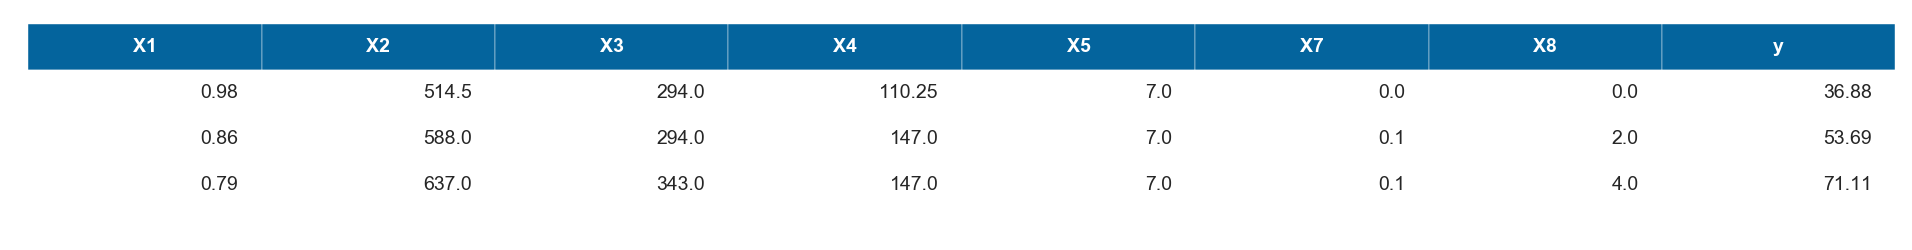
\includegraphics[scale=0.23]{../figures_trabalho_final/step_df.png}
      \captionof{}{DataFrame after csv read}
      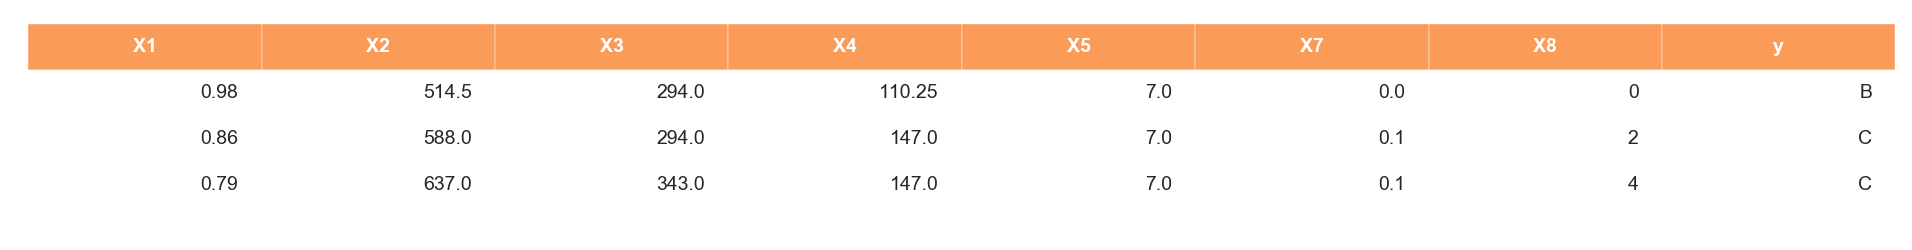
\includegraphics[scale=0.23]{../figures_trabalho_final/step_df_classif.png}
      \captionof{}{DataFrame for classification problem}
      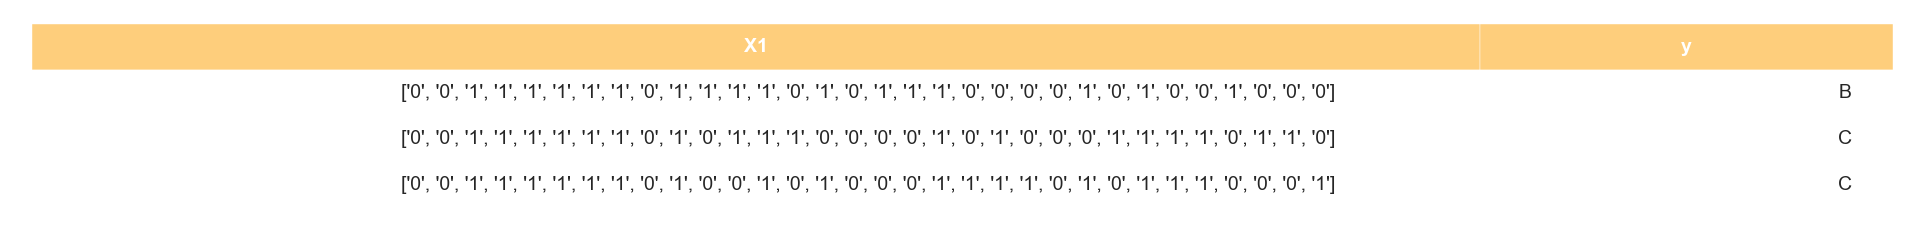
\includegraphics[scale=0.23]{../figures_trabalho_final/step_df_bin_classif.png}
      \captionof{}{DataFrame binarized for classification problem}
      \medskip
    \end{minipage}
\end{frame}

%-------------------------------------------------------
\subsection{Cross-Validation}
\begin{frame}{Introduction}{Cross-Validation}
Due to a lack of registers in the dataset, the use of cross-validation
with randomly choosen train and test sets where required for validation sake.
\bigskip
\begin{block}{Cross-Validation parameters}
\begin{itemize}
   \item For WiSARD parameters calibration : only 20 folds with $90\%$ for
     the training set and $10\%$ for the test set.
   \item For \textbf{overall} scores : 40 folds with $90\%$ for
     the training set and $10\%$ for the test set.
    \item The \textbf{accuracy} is then computed as the mean of all accuracies obtained
      over the folds.
\end{itemize}
\end{block}

\end{frame}

%-------------------------------------------------------
\section{CLassification Results}
%-------------------------------------------------------
\subsection{WiSARD parameters calibration}
\begin{frame}{Classification Results}{WiSARD parameters calibration}
%-------------------------------------------------------

\begin{minipage}{0.95\linewidth}
  \centering
  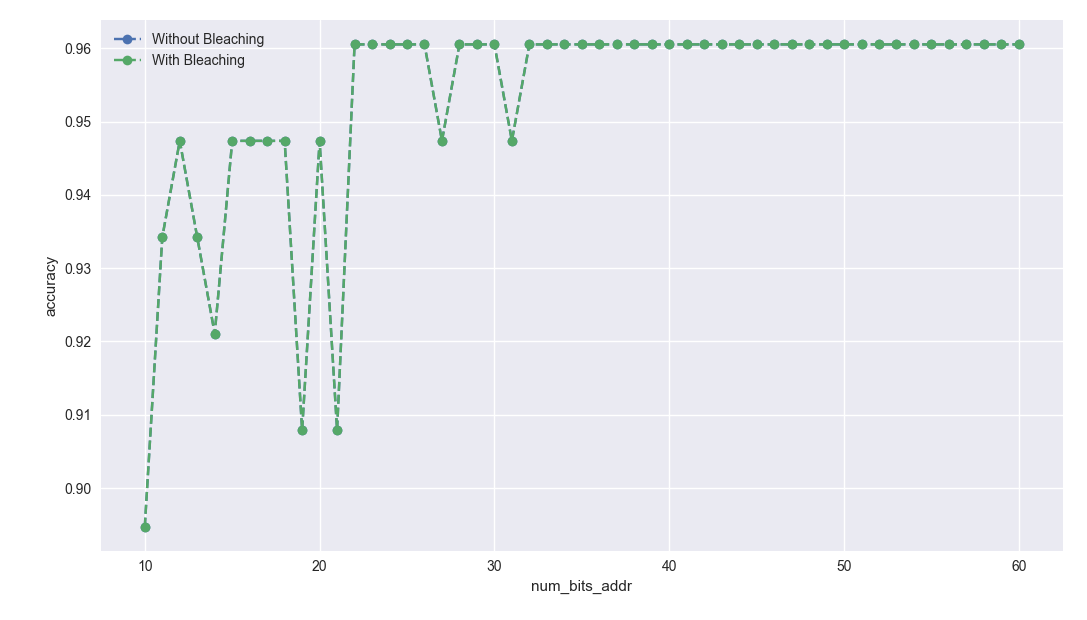
\includegraphics[scale=0.37]{../figures_trabalho_final/wisard_parameters_results.png}
  \captionof{}{num\_bits\_addr, bleaching}
  \medskip
\end{minipage}

\end{frame}

%-------------------------------------------------------
\subsection{WiSARD parameters calibration}
\begin{frame}{Classification Results}{Overall scores}
%-------------------------------------------------------

\centering
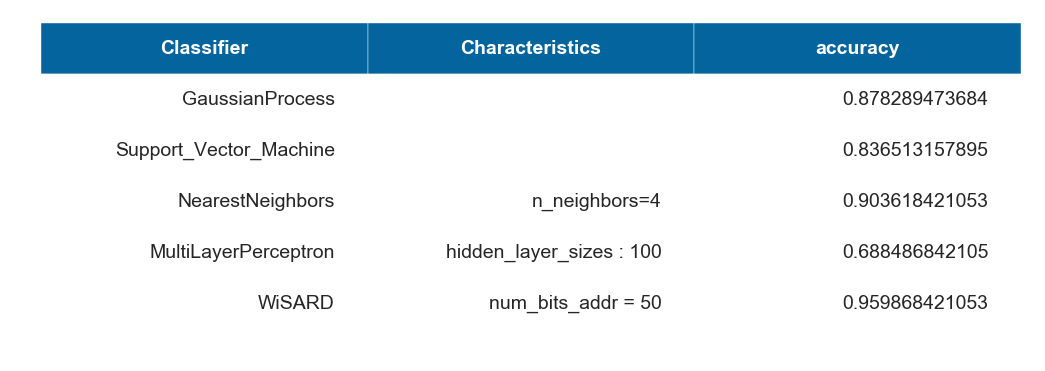
\includegraphics[scale=0.40]{../figures_trabalho_final/overall_results.png}
\captionof{}{overall}

\end{frame}

{\1
\begin{frame}[plain,noframenumbering]
  \finalpage{Thank you !}
\end{frame}}


\end{document}
